\documentclass[a4paper]{report}
\usepackage[english]{babel} 
\usepackage[utf8]{inputenc} 

\usepackage{amssymb,amsmath}
\usepackage{enumerate}
\usepackage{enumitem}

\usepackage{graphicx}
\usepackage{color,soul}
\usepackage{xcolor}

\definecolor{mygreen}{rgb}{0,0.6,0}
\definecolor{mygray}{rgb}{0.5,0.5,0.5}
\definecolor{mymauve}{rgb}{0.58,0,0.82}
\definecolor{greenish}{RGB}{105,114,41}

\usepackage[nottoc,numbib]{tocbibind}

\usepackage{xspace}

\usepackage{tikz}
\usetikzlibrary{arrows, automata, positioning}

\usepackage{parskip}

\usepackage{lmodern}
% \usepackage[
% 	text={To Be Approved},
% 	scale=0.8,
% 	angle=60
% ]{draftwatermark}

\usepackage[
	pdftex,
	pdfauthor={\@author},
	pdftitle={\@title},
	pdfsubject={},
	pdfkeywords={},
	pdfproducer={},
	pdfcreator={}
]{hyperref}
\hypersetup{
	colorlinks,
	linkcolor={red!50!black},
	citecolor={blue!50!black},
	urlcolor={blue!80!black}
}

\usepackage{pgfgantt}
\usepackage{lscape}

\usepackage{listings}

\lstset{
	backgroundcolor=\color{white},   % choose the background color; you must add \usepackage{color} or \usepackage{xcolor}; should come as last argument
	basicstyle=\ttfamily,        % the size of the fonts that are used for the code
	breakatwhitespace=true,          % sets if automatic breaks should only happen at whitespace
	breaklines=true,                 % sets automatic line breaking
	captionpos=b,                    % sets the caption-position to bottom
	commentstyle=\color{mygreen},    % comment style
	frame=single,	                 % adds a frame around the code
	keepspaces=true,                 % keeps spaces in text, useful for keeping indentation of code (possibly needs columns=flexible)
	columns=flexible,
	keywordstyle=\color{blue},   	 % keyword style
	commentstyle=\color{red},
	language=bash,                  % the language of the code
%	numbers=left,                    % where to put the line-numbers; possible values are (none, left, right)
%	numbersep=5pt,                   % how far the line-numbers are from the code
%	numberstyle=\tiny\color{mygray}, % the style that is used for the line-numbers
	rulecolor=\color{black},         % if not set, the frame-color may be changed on line-breaks within not-black text (e.g. comments (green here))
	showstringspaces=false,
	numberstyle=\small,
	stepnumber=1,                    % the step between two line-numbers. If it's 1, each line will be numbered
	stringstyle=\color{mymauve},     % string literal style
	tabsize=2,	                     % sets default tabsize to 2 spaces
	title=\lstname,                  % show the filename of files included with \lstinputlisting; also try caption instead of title
	morekeywords={match, where, return, --}
}

\newcommand{\lstlistshow}[2]{
	\begin{minipage}{\linewidth}
		\lstinputlisting[language=Dockerfile, caption={#2}]{#1}
	\end{minipage}
}

\newcommand{\lstlistdiscuss}[4]{
	\begin{minipage}{\linewidth}
		\lstinputlisting[language=Dockerfile, numbers=left, firstnumber=#2, linerange={#2-#3}, caption={#4}]{#1}
	\end{minipage}
}

\setlength\parindent{0pt}

\author{Claudio Bonesana}

\title{
    \Large New Techno War \\
	\rule{10cm}{0.3mm} \\
	\large \textit{Development guide} \\
	\begin{center}
		
\includegraphics[scale=0.8]{tank.png}
    \end{center}
}

\date{Last revision: \today}


\begin{document}
	
	\maketitle
	
	\tableofcontents
	
	% ---------------------------------------------------------------------------------------------------------
	
	\chapter{Introduction}

	This is development guide is intended to contains diagrams and explanation that are difficult to explain using in code comments.
	
	Although the majority of the code is covered by comments and follows a descriptive code-style, some diagrams are needed, hence the scope of this document.
	
	% ---------------------------------------------------------------------------------------------------------

	\chapter{GameManager utility class}

	This is an utility class. Its goal is to update the \texttt{GameState} in a definitive or not way. To manipulate in a safe way the \texttt{GameState}, use an instance of this class. This class does not contains any information: everything change is an update to the \texttt{GameState} object.

	For testing purposes, i.e. when an agent wants to see the consequences of an action, use the \texttt{activate()} method. This method will create \textit{a deep copy} of the \texttt{GameState} object before apply the changes to it.

	Otherwise, to apply in a definitive way the changes of an action to the state, use the \texttt{step()} method.

	The methods \texttt{buildMovements()}, \texttt{buildShoots()}, \texttt{buildResponses()}, \texttt{build\-ActionsForFigure()}, and \texttt{buildActions()} can be used to create different kind of actions.

	Other methods are used by the \texttt{MatchManager} class to control the development of a match.

	% ---------------------------------------------------------------------------------------------------------

	\chapter{MatchManager class state-machine}
	
	A \textit{match} is defined as following:

	\begin{itemize}
		\item The match is a collection of turns.
		\item In each turn the players activate all their units once and they can respond with their units at maximum once. First goes red player, then blue player.
		\item When all the figures are activated, the match goes to the next turn and the unit status is reset.
	\end{itemize}

	\begin{figure}[ht!]
		\centering
		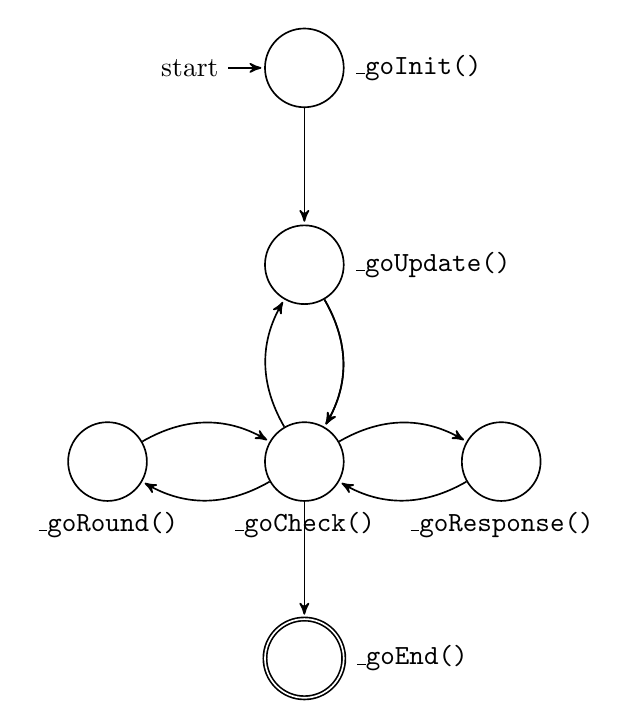
\begin{tikzpicture}[
			->,
			>=stealth',
			shorten >=1pt,
			auto,
			node distance=2.5cm,
			semithick,
			state/.style={circle, draw, minimum size=1cm}]
		]
			\tikzstyle{every state}=[fill={rgb:black,1;white,10}]

			\node[state,initial,label=right:\texttt{\_goInit()}] 	(Init)							{};
			\node[state,label=right:\texttt{\_goUpdate()}]			(Update)   	[below of=Init] 	{};
			\node[state,label=below:\texttt{\_goCheck()}]     		(Check)  	[below of=Update] 	{};
			\node[state,label=below:\texttt{\_goResponse()}]  		(Response)	[right of=Check] 	{};
			\node[state,label=below:\texttt{\_goRound()}]    		(Round)		[left of=Check] 	{};
			\node[state,accepting,label=right:\texttt{\_goEnd()}]	(End)		[below of=Check]  	{};

			\path[->]
			(Init)  	edge node				{} (Update)
			(Update) 	edge [bend left] node 	{} (Check)
			(Check) 	edge [bend left] node 	{} (Round)
						edge [bend left] node 	{} (Response)
						edge [bend left] node 	{} (Update)
						edge node 				{} (End)
			(Response)	edge [bend left] node 	{} (Check)
			(Round)		edge [bend left] node 	{} (Check)
			(Update)	edge [bend left] node 	{} (Check);
		\end{tikzpicture}
		\caption{State transition diagram of the MatchManager class.}
		\label{sd-mm}
	\end{figure}

	Figure~\ref{sd-mm} shows the state transition diagram of the \texttt{MatchManager} class. This class has the main purpose of manage a whole match. The structure of the match is decomposed into a state machine.
	
	For the creation of this object, it is required to pass as argument the \texttt{string value} of the classes to instantiate. This is a consequence of the web interface and the interaction with humans. Check the documentation of the \texttt{\_\_init\_\_()} method for further details.
	
	The state machine begin with an \textbf{initialization} step. Then the first action is an update action. After that, the state machine goes in \textit{check} mode: it checks the current status and decide where to go next. The possible outcomes are four: if there was a \textit{Shoot} or \textit{Move} action (but not a response), a \textbf{response} is possible; if there are still figures that can be activated, there will be a \textbf{round} step; if the goal of the scenario is achieved, then the match will \textbf{end}; otherwise, the only possible remaining state is a turn \textbf{update}. All other states step back to \textbf{check} with the exception of the \textbf{end} state.

	The class offers two utility methods:
	
	\begin{itemize}
		\item \texttt{nextStep()} will move the state-machine forward of one step.
		\item \texttt{nextTurn()} will move the state-machine forward until the turn change (an update happens).
	\end{itemize}

	% ---------------------------------------------------------------------------------------------------------

	\chapter{Players and Agents}

	The idea for the \textit{Agents} and the \textit{Players} is to use a common interface that can be easily used by the \texttt{MatchManager}. This interface is composed following methods:

	\begin{itemize}
		\item \texttt{chooseAction()},
		\item \texttt{chooseResponse()},
		\item \texttt{initialize()},
		\item \texttt{chooseFigureGroups()}.
	\end{itemize}

	Although the first two look similar, they need to be differentiated because the \textit{response} state offers the possibility to skip the generation of an action. This possibility is something that the Player or Agent need to keep in mind during the design stage.

	In the case that something is not doable, i.e. skip the \textit{response} action or if a figure does not have action doable, please raise the \texttt{ValueError} exception in order to inform the \textit{MatchManager} that there will not be an action available.

	There could be the possibility that some scenarios require an initialization step. In this step the Player or Agent need to think on how to setup their figures. There are three possible situations that need to be considered: the units are set; the units are already placed but the Player need to choose which positions to use; the units are not set but there is an area where the units can be placed.

	The methods \texttt{initialize()} and \texttt{chooseFigureGroups()} are intended to be used to fulfill this task and respectively initialize the units in a placement zone, or choose between groups of already placed units.

	Please, check the \texttt{agents.players.PlayerDummy} class for an example of implementation of a random player and on how to properly implement these functions.

	% ---------------------------------------------------------------------------------------------------------

	\bibliography{newtechnowar}{}
	\bibliographystyle{ieeetr}

\end{document}